\newpage
\section{Introduction}
Qu'est ce qu'une probabilité ? A quoi servent les probabilités ? 
Comment calculer une probabilité ? 
Dans ce chapitre nous nous attellerons à répondre à ces interrogations. \\

La théorie des probabilités est un ensemble d'outils mathématiques qui visent à 
quantifier l'incertitude d'un évènement. Par exemple, dans la vie de tous les jours : 
"Fera-t-il beau demain ?", "Est-ce que mon bus risque d'être en retard ?", 
"Est-ce que cette question risque de tomber à l'examen ?", etc... \\

Les probabilités permettent aussi de gérer des questions plus épineuses liées à la gestion 
de risque : "Le risque d'accident lié à un travail sur un circuit électrique à haute tension 
est-il élevé ?", "Quel est le risque d'avoir une inondation? Un feu de forêt ?", "Comment évolue une épidémie? "
 etc... \\

L'incertitude doit être prise en compte dans la planification.

Santé, nourriture, emploi, économie... les probabilités apparaissent même dans les fondements des lois de la nature. En effet, 
en mécanique quantique on calcule des probabilités de présence des particules à tel ou 
tel endroit ou encore la probabilité qu'une particule aie telle ou telle vitesse ! \\

Enfin, les probabilités sont également les fondements des techniques de machine learning. 
Comment fonctionnent les algorithmes de suggestions de YouTube, Netflix ou Spotify?
Comment peut-on analyser des images médicales de manière automatique ?


Statistiques et probabilités nous aide à comprendre et travailler avec l'incertain. 
Là où les statistiques s'occupent de recueillir et d'analyser les données du monde réel, 
les probabilités apportent 
la base mathématique théorique, construisent des modèles idéaux, permettant aux statistiques de fonctionner.\\
Toutes les notions qui ont été vues en statistiques précédemment peuvent être reliées à des notions de probabilités.
Dans beaucoup de cas, en statistiques on "estime" des quantités définies en probabilités.\\
\\~
\begin{figure}
    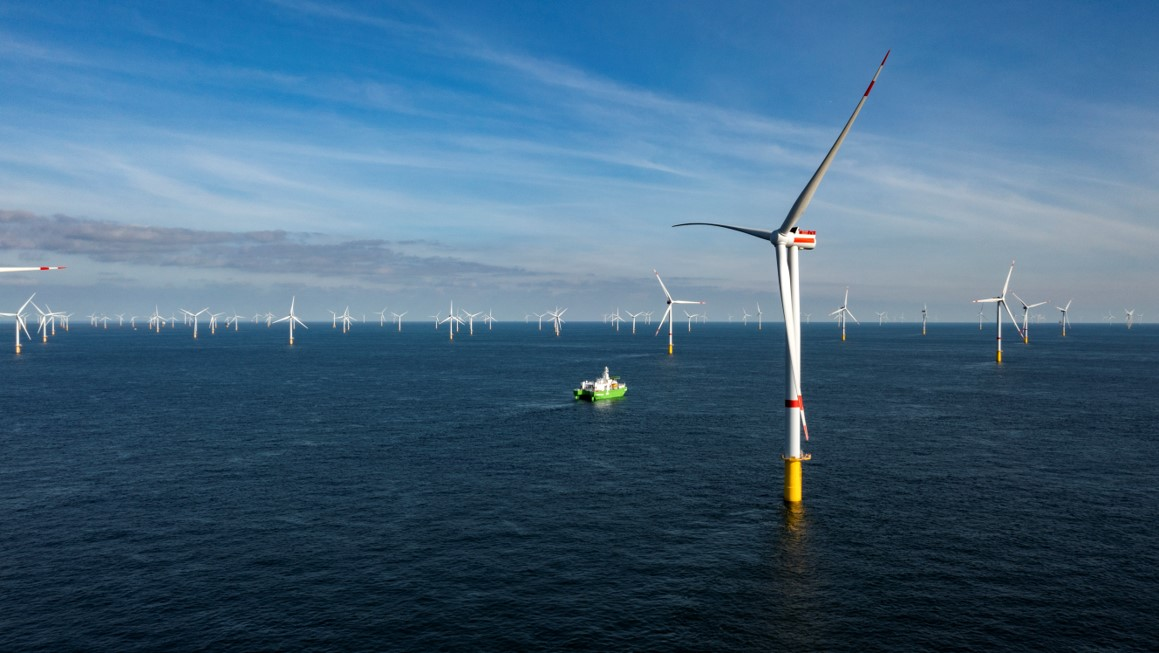
\includegraphics[scale=0.7]{./images/eolienne.jpg}
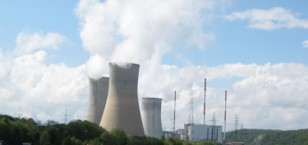
\includegraphics[scale=0.9]{./images/nuclear.jpg}\\
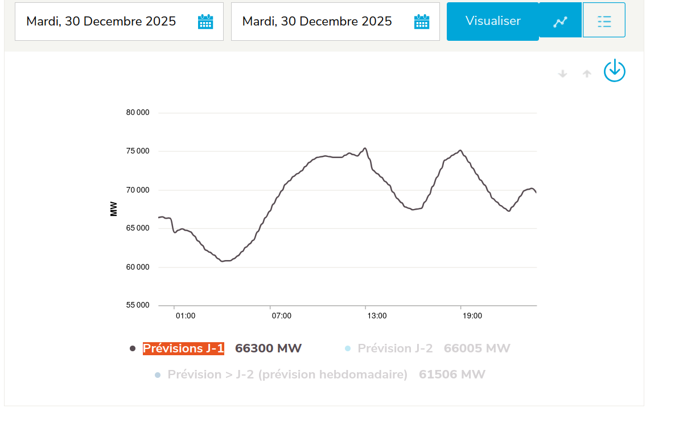
\includegraphics[scale=0.7]{./images/elec.png}
\caption{Production d'électricité, prédiction de la demande.}
\end{figure}
\begin{figure}
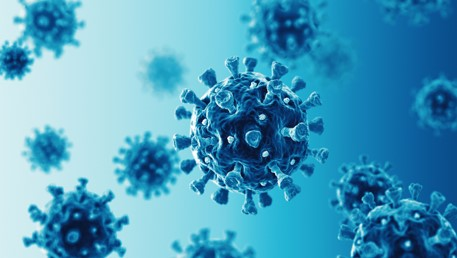
\includegraphics[scale=0.3]{./images/virus.jpg}
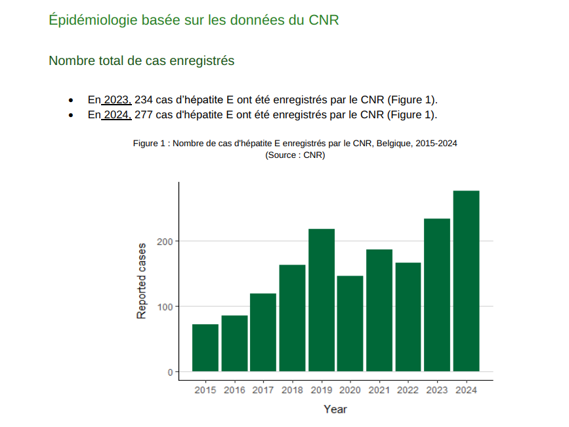
\includegraphics[scale=0.7]{./images/hepatite.png}\\
\caption{Suivi, recueil de données, modélisation des épidémies.}
\end{figure}
\begin{figure}
    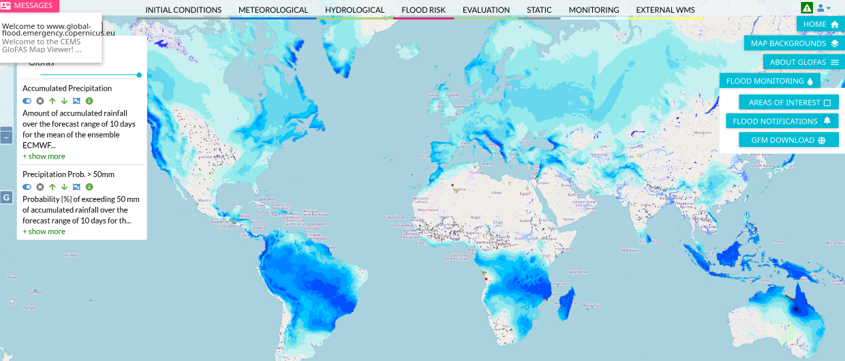
\includegraphics[scale=0.7]{./images/inondations.png}\\
    \caption{Gestion des inondations, prédictions.}
\end{figure}
\begin{figure}
    \centering
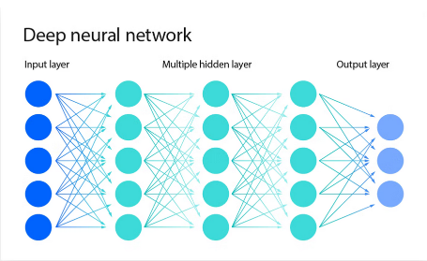
\includegraphics[scale=0.7]{./images/ml.png}\\
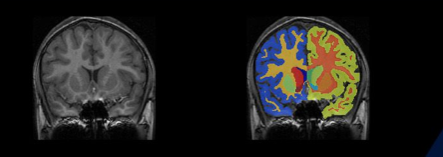
\includegraphics[scale=0.7]{./images/mri.png}\\

\includegraphics[scale=0.7]{./images/netflix.png}

\includegraphics[scale=0.7]{./images/spotify.png}

    \caption{Machine learning.}
\end{figure}


